% Szymon
\section{Kolorowania węzłów}

 Głównym zadaniem teorii węzłów jest stworzenie narzędzi służących do opisywania, klasyfikowania oraz rozróżniania węzłów. Na podstawie twierdzenia przedstawionego w poprzedniej części wiemy że, diagramy są równoważne jeżeli pierwszy można przekształcić do drugiego stosując ruchy Reidemeistera. Sprawdzanie równoważności diagramów w ten sposób jest jednak uciążliwe, oraz czasochłonne.  W niniejszej części zostanie przedstawione zagadnienie kolorowania diagramów węzłów. Kolorowanie węzłów jest niezmiennikiem diagramu. Oznacza to że gdy pierwszy diagram posiada pewną własność kolorowania, a drugi nie, to diagramy te nie są równoważne, a więc przedstawiają różne węzły. Kolorowanie nie jest idealnym narzędziem klasyfikującym i istnieją diagramy nierównoważne o takich samych własnościach kolorowania. \\
 Kolejność omawianych zagadnień w tym rozdziale będzie następująca: Najpierw podana zostanie definicja kolorowania, oraz warunki które muszą zostać spełnione aby węzeł mógł zostać w określony sposób pokolorowany. Następnie zdefiniowane zostaną równania kolorowań oraz macierze kolorowań. Kolejnym etapem będzie wprowadzenie macierzy kolorowań jako niezmiennika węzłów. Ostatnią część stanowić będzie wskazanie relacji pomiędzy klasami diagramów węzłów a grupami kolorowań.

\subsection{Kolorowanie diagramów}

Niech K będzie węzłem zorientowanym, L jego diagramem, B = $\lbrace b_{1}, \ldots, b_{k}\rbrace$ zbiorem łuków,  C = $\lbrace c_{1}, \ldots, c_{k}\rbrace$ zbiorem skrzyżowań. 

\begin{definicja}
Diagram L jest kolorowalny modulo $n \in \N$, gdy każdemu łukowi diagramu L można przyporządkować liczbę $a \in \lbrace 0, \ldots, n-1 \rbrace$ w taki sposób, że: \\ \\
	\begin{minipage}{0.7\textwidth}
	
	\begin{enumerate}
		\item Dla każdego skrzyżowania $c_{j}$ spełnione jest równanie kolorowania \\ $a_{2}+a_{3}-2a_{1} \equiv 0$ mod n
		\item Kolorowanie nie jest stale, tzn istnieją łuki $b_{i}, b_{j}$ którym 			przyporządkowano różne liczby.
		 
	\end{enumerate}
	\end{minipage}
	\begin{minipage}{0.3\textwidth}
	\begin{center}

	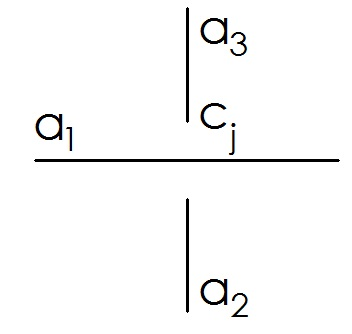
\includegraphics[scale=0.35]{2/Obrazy/Crossing1}
	\end{center}
	\end{minipage}
\end{definicja}
Przyporządkowanie spełniające powyższe własności nazywa się \emph{kolorowaniem diagramu mod n}.




\begin{twierdzenie} Kolorowalność modulo n jest niezmiennikiem węzła.
\end{twierdzenie}
\begin{proof}
Dwa diagramy $L_{1}, L_{2}$ są równoważne jeżeli istnieje ciąg ruchów Reidemeistera przekształcający $L_{1}$ w $L_{2}$. Wystarczy zatem sprawdzić że kolorowalność modulo n nie zmienia się po wpływem ruchów Reidemeistera.

\begin{enumerate} \item Pierwszy ruch Reidemeistera: 

	\begin{minipage}{0.5\textwidth}
	Dla skrzyżowania $c_{j}$ spełnione jest równanie \\ $a_{1}+a_{2}-2a_{2} \equiv 0$ mod n. Zatem $a_{1} \equiv a_{2}$.
	\end{minipage}
	\begin{minipage}{0.5\textwidth}
		\begin{center}
			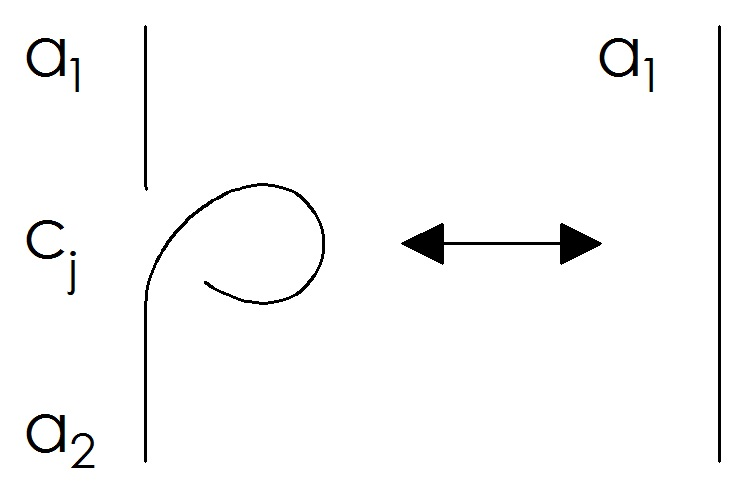
\includegraphics[scale=0.2]{2/Obrazy/R1}
		\end{center}
	\end{minipage}
\item Drugi ruch Reidemeistera: 

	\begin{minipage}{0.5\textwidth}
	Dla skrzyżowania $c_{j1}$ mamy \\ $a_{1}+a_{4}-2a_{2} \equiv 0$ mod n.\\ Dla skrzyżowania $c_{j2}$, \\$a_{3}+a_{4}-2a_{2} \equiv 0$ mod n. \\Stąd $a_{1} \equiv a_{3} $ mod n.
	\end{minipage}
	\begin{minipage}{0.5\textwidth}
		\begin{center}
			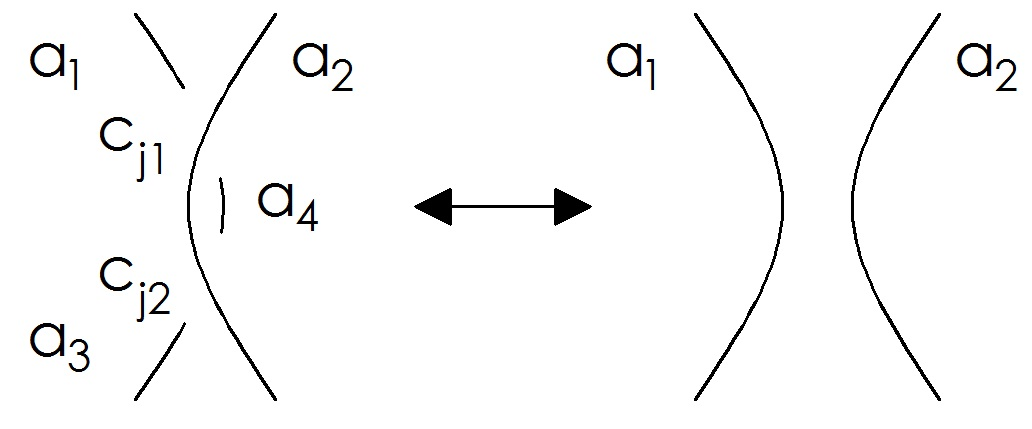
\includegraphics[scale=0.2]{2/Obrazy/R2}
		\end{center}
	\end{minipage}
	
\item Trzeci ruch Reidemeistera: 


	Dla skrzyżowania $c_{j2}$ mamy $a_{5}+a_{2}-2a_{3} \equiv 0$ mod n. Analogicznie dla skrzyżowania $c_{j5}$, $a_{8}+a_{2}-2a_{3} \equiv 0$ mod n. Stąd $a_{8} \equiv a_{5}$ mod n. \\ \\
	\begin{minipage}{0.35\textwidth}
	W drugim przypadku mamy:\\
	$a_{4} \equiv 2a_{2}-a_{1}$. \\
	$a_{6} \equiv 2a_{3}-a_{4} \equiv$ \\$\equiv 2a_{3}-2a_{2}+a_{1} $.	\\
	$a_{8} \equiv 2a_{3}-a_{2}$. \\	
	$a_{7} \equiv 2a_{3}-a_{1}$.\\		
	$a_{9} \equiv 2a_{8}-a_{7} \equiv$ \\$\equiv 2a_{3}-2a_{2}+a_{1} \equiv a_{6} $. \\
	\end{minipage}
	\begin{minipage}{0.65\textwidth}
		\begin{center}
			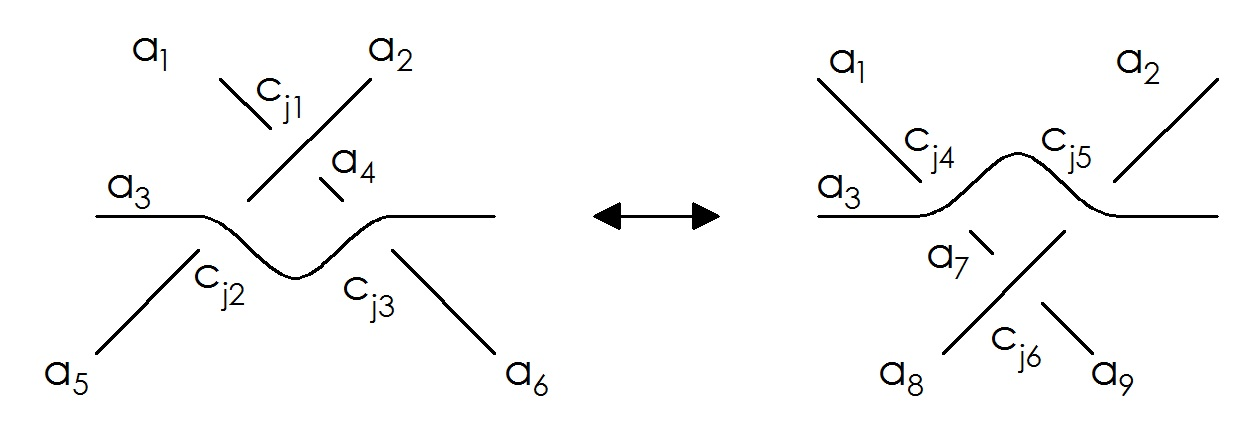
\includegraphics[scale=0.25]{2/Obrazy/R3}
		\end{center}
	\end{minipage}
	Zatem, kolory łuków o indeksach różnych od 7 nie ulegają zmianie. Kolor łuku $a_{7}$ zmienia się i wynosi $a_{7} \equiv a_{6} - a_{2} + a_{4}$. Wtedy otrzymane kolorowanie spełnia równania kolorowań w diagramie $L_{2}$.
\end{enumerate}
\end{proof}


\begin{definicja}
Niech B = $\lbrace b_{1}, \ldots, b_{k}\rbrace$ będzie zbiorem łuków. Kolorowaniem $(a_{b_{1}}, \ldots, a_{b_{k}})$ nazywamy przyporządkowanie każdemu łukowi $b_{i}$ koloru $a_{b{i}}$, tak aby spełnione były równania kolorowań. W dalszej części opracowania zapis ten zostanie uproszczony do postaci $(a_{1}, \ldots, a_{k})$, gdzie indeks przy $a$, odpowiada numerowi łuku, którego ten kolor dotyczy.
\end{definicja}


\begin{lemat}
Jeżeli dla diagramu L istnieje kolorowanie $( a_{1}, \ldots , a_{k} )$, to dla każdego l $\in \N\:\: ( a_{1}+l, \ldots , a_{k}+l )$ też jest kolorowaniem.
\end{lemat}
\begin{proof}
Dla każdego $c_{j}$ spełnione jest:\\
$a_{m_{1}}+a_{m_{2}}-2a_{m_{3}} \equiv 0$ mod n. Wobec czego \\ 
$a_{m_{1}}+l+a_{m_{2}}+l-2a_{m_{3}}-2l \equiv 0$.
\end{proof}
\textbf{Wniosek:} Jeśli diagram jest kolorowalny to istnieje kolorowanie takie że $a_{1} = 0$.

\paragraph{Kolorowanie modulo 2} Jeżeli węzeł jest kolorowalny modulo 2 to dla każdego skrzyżowania zachodzi jedna z czterech możliwości:
	\begin{center}
			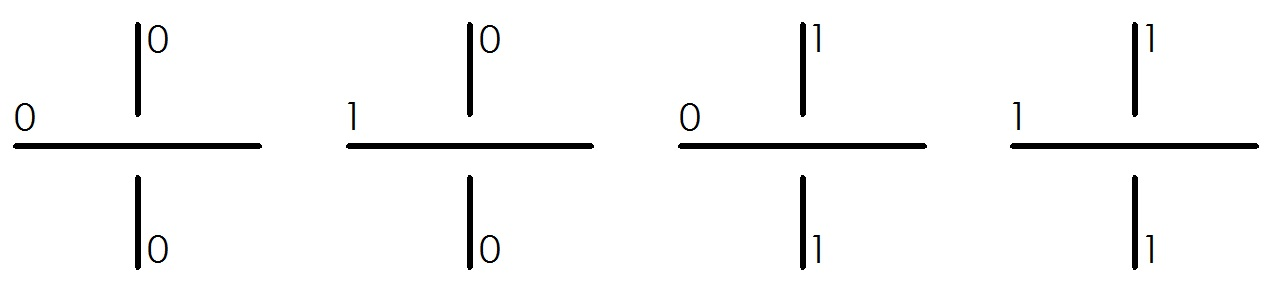
\includegraphics[scale=0.3]{2/Obrazy/Mod2}
	\end{center}
	W każdym przypadku kolory łuków leżących po przeciwnych stronach skrzyżowania są jednakowe. Startując w dowolnym punkcie węzłą i przechodząc go w wybranym kierunku otrzymamy że każdy łuk należący do tej samej komponenty spójności co punkt startowy ma przyporządkowany jednakowy kolor. Zatem splot może być kolorowany mod 2 $\Leftrightarrow$ splot składa się z co najmniej 2 węzłów.
	
	\begin{definicja}
	Niech K będzie splotem, L jego diagramem. Diagram L jest podzielny jeśli splot składa się z co najmniej 2 węzłów, oraz  $\exists U, V\:  otwarte, U \cap V = \emptyset$, takie że $ L\subseteq U\cup V, L\cap U \neq \emptyset, L\cap V \neq \emptyset$.
	\end{definicja}
	
	
\begin{lemat}
	Jeżeli splot K jest podzielny to, $\forall n >1 \:\:$ diagram L jest kolorowalny mod n.
\end{lemat}
	
\begin{proof}
Niech każdy łuk zawarty w U będzie pokolorowany na kolor 0, łuk zawarty w V na kolor 1. Takie przyporządkowanie jest kolorowaniem. Równania skrzyżowań zachodzą dla każdego n. 
\end{proof}


	
\subsection{Równania kolorowań}
\begin{definicja}
Krótki łuk, to część łuku który przechodzi dokładnie przez 2 skrzyżowania. 
\end{definicja}
Przykład: Łuk $b_{1}$ przechodzi przez 5 skrzyżowań i składa się z 4 krótkich łuków. \\

\begin{center}
			\includegraphics[scale=0.2]{2/Obrazy/ShortArc} \\
\end{center}

\begin{definicja}
Region to komponenta spójności $\R^{2} \setminus L$.
\end{definicja}
\begin{definicja}
Szachownica diagramu to przyporządkowanie każdemu regionowi jednego z 2 kolorów tak aby każdy krótki łuk oddzielał regiony o różnych kolorach.
\end{definicja}

\textbf{Przykład:} Rozważmy węzeł który w literaturze jest oznaczony symbolem $7_{3}$. Diagram węzła jest przedstawiony na rysunku poniżej (pierwszy z lewej). Węzeł posiada 7 łuków, 14 krótkich łuków, oraz 9 regionów.

			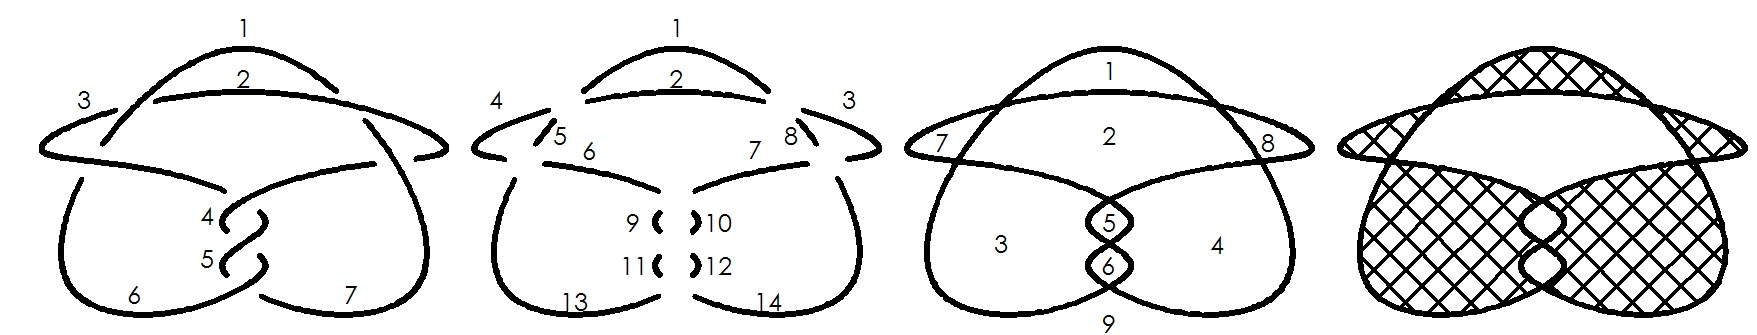
\includegraphics[scale=0.3]{2/Obrazy/ArcRegion3} \\



\begin{lemat}
Dla każdego węzła K istnieje szachownica jego diagramu.  
\end{lemat}
\begin{proof}
Ustalmy węzeł K, oraz jego diagram L. Niech $L$ będzie zawarty w pewnej kuli otwartej $\Omega$.
Weźmy dowolny region diagramu L. Ustalmy punkt P należący do tego regionu. Weźmy dowolne dwie krzywe o następujących własnościach:




	\begin{minipage}{0.5\textwidth}
\begin{itemize}
\item Krzywe są bez samo przecięć i nie przecinają się wzajemnie,
\item Początki krzywych znajdują się w punkcie P,
\item Końce krzywych znajdują się na brzegu $\Omega$,
\item Krzywa nie przechodzi przez skrzyżowania.	
\end{itemize}
	\end{minipage}
	\begin{minipage}{0.5\textwidth}
		\begin{center}
			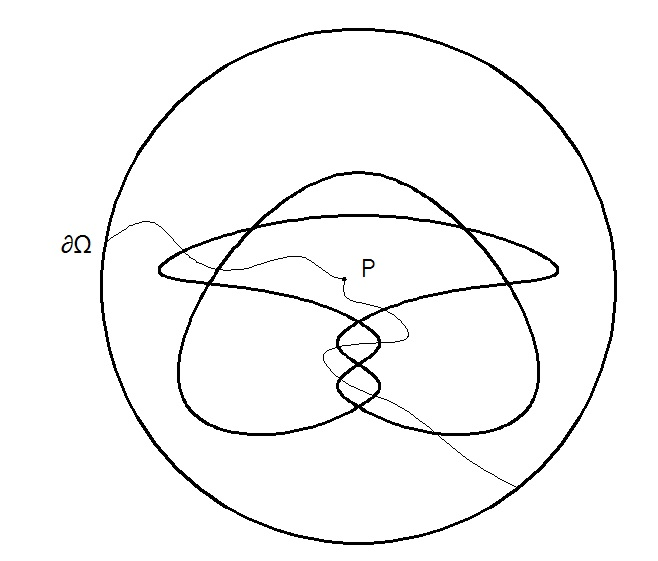
\includegraphics[scale=0.3]{2/Obrazy/Chesscircle}
		\end{center}
	\end{minipage}
Zatem suma krzywych dzieli węzeł na 2 części. Ponadto obie krzywe przecinają parzystą liczbę łuków. Zatem każda z krzywych przecina taką samą liczbę łuków modulo 2. Stąd kolor regionu nie zależy od wyboru krzywej, więc szachownica diagramu istnieje zawsze. 

\end{proof}
Dla każdego skrzyżowania $c_{j}$ równanie można przedstawić na 2 sposoby. 

\begin{definicja}
Wybór znaku równania kolorowania nazywa się dobrym, gdy przyjmuje następującą postać: 
\end{definicja}

	\begin{minipage}{0.5\textwidth}
$a_{m2}+a_{m3}-2a_{m1} \equiv 0$ mod n, dla \\	
	\begin{center}
			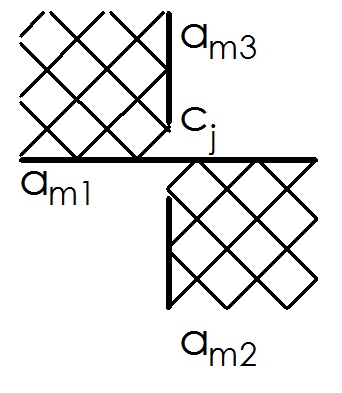
\includegraphics[scale=0.3]{2/Obrazy/Cros+}
	\end{center}
	\end{minipage}
	\begin{minipage}{0.5\textwidth}
$2a_{m1}-a_{m2}-a_{m3} \equiv 0$ mod n, dla \\
	\begin{center}
			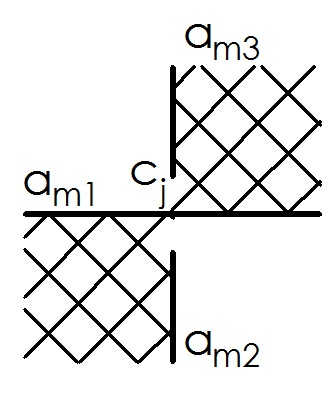
\includegraphics[scale=0.3]{2/Obrazy/Cros-}
	\end{center}	
	\end{minipage}

\begin{lemat}
Suma równań po wszystkich skrzyżowaniach równa się 0, o ile znaki równań zostały \emph{wybrane dobrze}.
\end{lemat}
\begin{proof}
Ustalmy dowolny łuk $b_{j}$, z kolorem  $a_{j}$. Łuk $b_{j}$ składa się z pewnej liczby krótkich łuków $b_{j}^{i}$. Każdy krótki łuk łączy dokładnie 2 skrzyżowania. Istnieje region $X_{i}$, taki że oba skrzyżowania graniczą z $X_{i}$. Niech $a_{j}^{i}$ oznacza kolor $b_{j}^{i}$ krótkiego łuku. Kolor każdego krótkiego łuku występuje w równaniach dokładnie 2 skrzyżowań.
\begin{center}
  			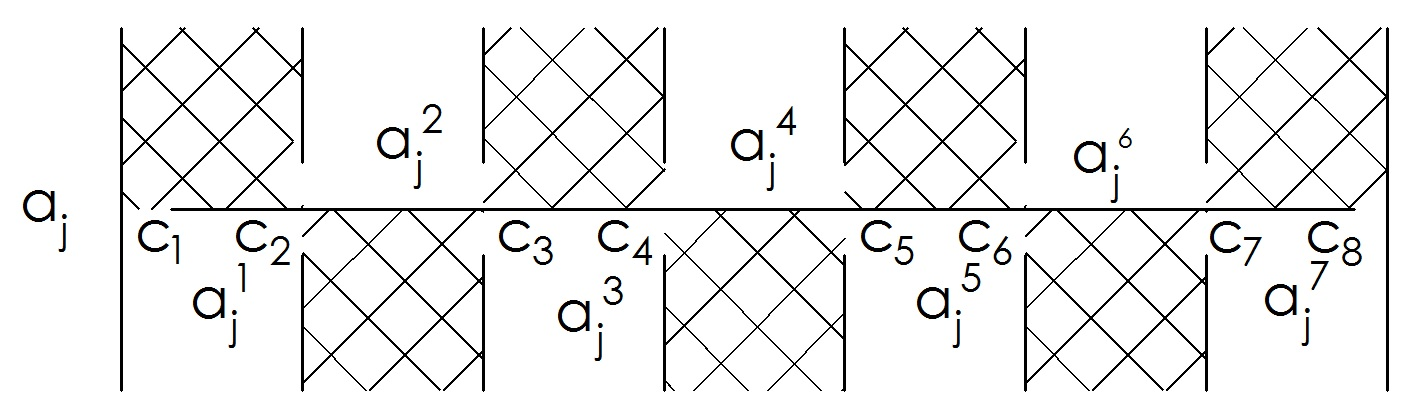
\includegraphics[scale=0.3]{2/Obrazy/zerosum2}
\end{center}
Ponieważ znaki równań zostały  \emph{wybrane dobrze}, znak $a_{j}^{i}$ w równaniu skrzyżowania  
$c_{j1}$, jest przeciwny do znaku $a_{j}^{i}$ w równaniu skrzyżowania $c_{j2}$. Wobec czego równania dla krótkich łuków sumują się do 0, dla każdego i. Zatem sumują się również do 0 dla równań kolorowań zwykłych łuków.
\end{proof}

\textbf{Wniosek:} Niech łuk j, ma początek w skrzyżowaniu $c_{m}$. Zaczynając w $c_{m}$ a następnie idąc wzdłuż łuku i sumując współczynniki przy j-tym łuku w mijanych równaniach skrzyżowań, suma zawsze wynosi $\pm 1$.
\begin{proof}
Zamiast sumować współczynniki przy j-tym łuku w kolejnych równaniach skrzyżowań można sumować współczynniki przy odpowiadających mu krótkich łukach. Z lematu współczynniki sumują się do 0. Zatem suma wszystkich współczynników jest równa współczynnikowi krótkiego łuku przy ostatnim mijanym skrzyżowaniu, a ten współczynnik wynosi $\pm 1$.

\end{proof}

\begin{comment}
\begin{lemat}
Dla każdego  każdego łuku j można tak wybrać znaki dla każdego skrzyżowania dla każdego skrzyżowania, że suma równań po wszystkich skrzyżowaniach równa się 0, oraz suma współczynników przy łuku j po skrzyżowaniach ze zbioru W równa się $\pm 1$.
\end{lemat}

\begin{proof}

\end{proof}
\end{comment}

\subsection{Macierze kolorowań}
\begin{definicja}
Łuk zamknięty w diagramie to węzeł składający się dokładnie z jednego łuku.
\end{definicja}
\begin{center}
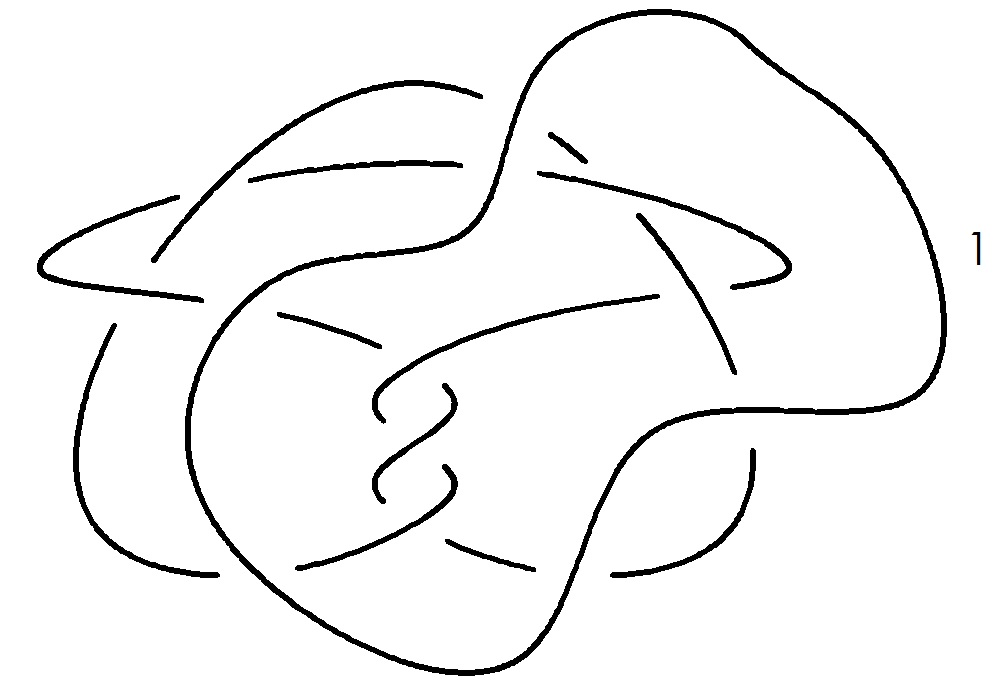
\includegraphics[scale=0.2]{2/Obrazy/Clossedcurve} \\

\end{center}

\begin{lemat}
Jeżeli węzeł K nie zawiera łuków zamkniętych, to liczba skrzyżowań i łuków w diagramie L jest równa .
\end{lemat}
\begin{proof}
Niech L będzie diagramem zorientowanym. Ponieważ węzeł nie zawiera łuków zamkniętych to dla każdego łuku istnieją dokładnie 2 skrzyżowania które odpowiadają początkowi i końcowi łuku. Dodatkowo każde skrzyżowanie jest początkiem i końcem dokładnie 2 łuków. Zatem funkcja przyporządkowywująca łukowi skrzyżowanie będące jego początkiem jest bijekcją.
\end{proof}


Niech L będzie diagramem bez łuków zamkniętych, B zbiorem łuków, $( a_{1}, \ldots, a_{k})$ jego kolorowaniem modulo n, C zbiorem skrzyżowań.  
\begin{definicja}
Macierz kolorowania $A_{+}$ to macierz powstała ze współczynników występujących w równaniach kolorowań diagramu L, przy czym znaki równań kolorowań zostały wybrane dobrze. $A_{+}=(a_{ij})$, gdzie  $a_{ij}$ odpowiada współczynnikowi przy kolorze i-tego łuku w równaniu $c_{j}$-tego skrzyżowania. 
\end{definicja}
Proces tworzenia macierzy $A_{+}$, dla węzła $7_{3}$ został przedstawiony poniżej. \\

	\begin{minipage}{0.5\textwidth}

	\begin{center}
			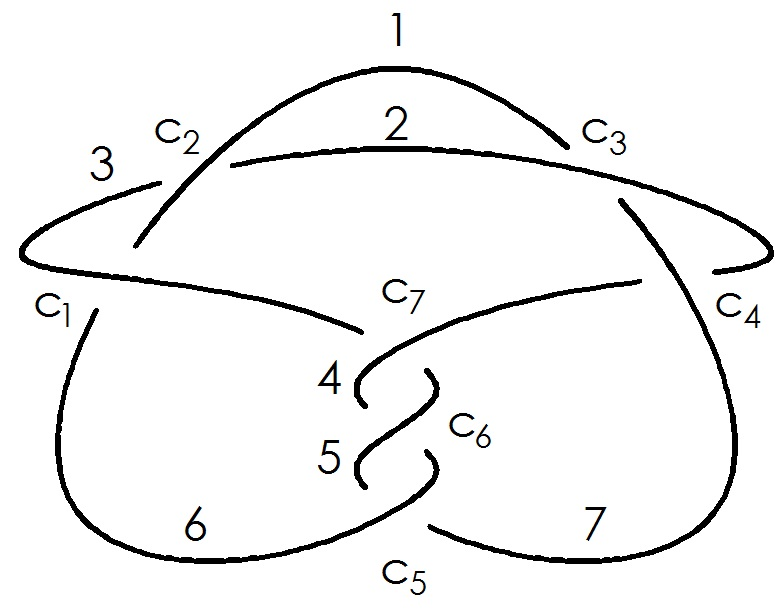
\includegraphics[scale=0.3]{2/Obrazy/73matrix}
	\end{center}
	\end{minipage}
	\begin{minipage}{0.5\textwidth}

	\begin{center}
			$c_{1}: \quad a_{1} + a_{6} - 2a_{3} \equiv 0 $ mod n
			$c_{2}: \quad a_{2} + a_{3} - 2a_{1} \equiv 0 $ mod n
			$c_{3}: \quad a_{1} + a_{7} - 2a_{2} \equiv 0 $ mod n	
			$c_{4}: \quad a_{2} + a_{4} - 2a_{7} \equiv 0 $ mod n	
			$c_{5}: \quad a_{5} + a_{7} - 2a_{6} \equiv 0 $ mod n	
			$c_{6}: \quad a_{4} + a_{6} - 2a_{5} \equiv 0 $ mod n	
			$c_{7}: \quad a_{3} + a_{5} - 2a_{4} \equiv 0 $ mod n	
	\end{center}	
	\end{minipage}
	
\begin{center}


$\newline A_{+} = \bordermatrix { ~ & 1 & 2 & 3 & 4 & 5 & 6 & 7  \cr
					c_{1} & 1 & 0 &-2 & 0 & 0 & 1 & 0	 \cr
					c_{2} &-2 & 1 & 1 & 0 & 0 & 0 & 0  \cr
					c_{3} & 1 &-2 & 0 & 0 & 0 & 0 & 1  \cr
					c_{4} & 0 & 1 & 0 & 1 & 0 & 0 &-2  \cr
					c_{5} & 0 & 0 & 0 & 0 & 1 &-2 & 1  \cr
					c_{6} & 0 & 0 & 0 & 1 &-2 & 1 & 0  \cr
					c_{7} & 0 & 0 & 1 &-2 & 1 & 0 & 0  \cr} $

\end{center}
$\newline$
\textbf{Obserwacja:} Równania kolorowań diagramu L są liniowo zależne, bo sumują się do 0. Zatem wyznacznik macierzy kolorowania $\vert det  \big(A_{+}\big) \vert = 0$.
  
  \begin{definicja}
	Macierz kolorowań $A$ wymiaru $(k-1) \times (k-1)$, to dowolny minor macierzy $A_{+}$ powstały poprzez usunięcie jednego wiersza i jednej kolumny.
  \end{definicja}
    \begin{definicja}
    Wyznacznik diagramu $ det \big(L\big)$ to moduł z wyznacznika $\vert det \big(A\big) \vert$.
    \end{definicja}
    
\begin{twierdzenie}
Wyznacznik diagramu jest dobrze określony, nie zależy od wyboru minora macierzy $A_{+}$
\end{twierdzenie}

\begin{proof}
Niech $A_{i,j}$ oznacza minor powstały poprzez usunięcie i-tego wiersza, oraz j-tej kolumny. W macierzy $A_{+}$ suma elementów w wierszu, oraz suma elementów w kolumnie równa się 0, ponieważ znaki równań są wybrane dobrze. Niech X będzie macierzą $k \times k$, oraz X = 
$
\begin{pmatrix}
 1 & \cdots & 1 \\
 \vdots & \ddots & \vdots \\
 1 & \cdots & 1 \\
\end{pmatrix}
$. Rozważmy \\
\begin{center}
 $det\big( A_{+}+X \big)=det \begin{pmatrix}
 1+a_{1,1} & \cdots & 1+a_{1,k} \\
 \vdots & \ddots & \vdots \\
 1+a_{k,1} & \cdots & 1+a_{k,k} \\
\end{pmatrix}$ \\
\end{center} 
Suma elementów w każdej kolumnie, oraz w każdym wierszu równa się k. Wyznacznik zostanie obliczony w następujących krokach:
\begin{enumerate}
\item Po dodaniu do  i-tego wiersza, sumy pozostałych wierszy każdy element i-tego wiersza będzie mieć wartość k. Wartości w pozostałych komórkach pozostaną niezmienione. \\
\begin{center}

$det \begin{pmatrix}
 1+a_{1,1} & \cdots &  1+a_{1,k} \\
 \vdots & \ddots & \vdots \\
  k & \cdots &  k \\ 
 \vdots & \ddots & \vdots \\
 1+a_{k,1} & \cdots & 1+a_{k,k} \\
\end{pmatrix}$ \\
\end{center}

\item Po dodaniu do j-tej kolumny, sumy pozostałych kolumn, element $a_{i,j}$ będzie mieć wartość $k^2$. Pozostałe elementy w i-tym wierszu, oraz j-tej kolumnie będą mieć wartość k. Pozostałe elementy pozostaną niezmienione. \\
\begin{center}
$det \begin{pmatrix}
 1+a_{1,1} & \cdots & k & \cdots &  1+a_{1,k} \\
 \vdots & \ddots & \vdots & \ddots & \vdots \\
  k & \cdots & k^2 & \cdots & k \\ 
 \vdots & \ddots & \vdots & \ddots & \vdots \\
 1+a_{k,1} & \cdots & k & \cdots &  1+a_{k,k} \\
\end{pmatrix}$ \\
\end{center}

\item Po wyciągnięciu k przed wyznacznik, wyrażenie będzie miało postać. \\
\begin{center}
$k \times det \begin{pmatrix}
 1+a_{1,1} & \cdots & k & \cdots &  1+a_{1,k} \\
 \vdots & \ddots & \vdots & \ddots & \vdots \\
  1 & \cdots & k & \cdots & 1 \\ 
 \vdots & \ddots & \vdots & \ddots & \vdots \\
 1+a_{k,1} & \cdots & k & \cdots &  1+a_{k,k} \\
\end{pmatrix}$ \\
\end{center}
\item Odejmując i-ty wiersz od pozostałych wierszy otrzymamy. 
\begin{center}
$k \times det \begin{pmatrix}
 a_{1,1} & \cdots & 0 & \cdots &  a_{1,k} \\
 \vdots & \ddots & \vdots & \ddots & \vdots \\
  1 & \cdots & k & \cdots & 1 \\ 
 \vdots & \ddots & \vdots & \ddots & \vdots \\
 a_{k,1} & \cdots & 0 & \cdots &  a_{k,k} \\
\end{pmatrix}$ \\
\end{center}

Korzystając z rozwinięcia Lalpace'a względem j-tej kolumny: \\ $\vert det  \big(A+X \big) \vert = k^2 \times \vert (-1)^{i+j} \times det \big( A_{i,j} \big) \vert$, dla każdego $i, j$. Zatem $\vert det \big( A_{i,j} \big) \vert$ nie zależy do wyboru $i, j$. 

\end{enumerate}


\end{proof}



\subsection{Własności wyznacznika diagramu}
Wyznacznik diagramu jest powiązany z możliwymi kolorowaniami diagramu.

\begin{lemat}
Niech A będzie macierzą o wyrazach całkowitych. Istnieją macierze X, Y o wyrazach całkowitych, takie że $\vert det(X) \vert= \vert det(Y) \vert=1$, oraz macierz diagonalna $\vert D \vert=(\vert d_{i,i} \vert)$, taka że $D=XAY$.
\end{lemat}
\begin{proof}
Niech A będzie macierzą wymiaru $k \times k$, oraz  $a$ liczbą całkowitą. Ustalmy macierze:
\begin{itemize}
\item $Z^1_{i,j}$  -  Macierz odpowiadająca transpozycji i-tej, oraz j-tego wektora macierzy A,

\item $Z^2_{i,aj}$ -  Macierz odpowiadająca dodaniu do  i-tego wektora, a-tą krotność j-tego wektora.
\end{itemize}
Każda z powyższych macierzy ma wyznacznik 1. \\
$\textbf{Krok 1:}$ Mnożąc macierz $A$ z lewej lub prawej przez $Z^1$ da się 
ją przekształcić do postaci $A^{(1)}$, takiej że najmniejszy co do modułu, niezerowy wyraz znajduje się w lewym górnym rogu macierzy. Następnie mnożąc z lewej lub prawej przez 
$Z^2_{i,a1}$, można przekształcić macierz do postaci $A^{(2)}$ takiej że, wartość bezwzględna każdego elementu leżącego w pierwszym wierszu lub pierwszej kolumnie jest mniejsza od wartości bezwzględnej elementu $a_{1,1}$. \\
$\textbf{Krok 2:}$ Powtarzając Krok 1, można sprowadzić macierz do postaci 
\begin{center}
$A^{(n_{1})}=\begin{pmatrix}
a_{1,1} & 0 & \cdots & 0 \\
0 & a_{2,2} & \cdots & a_{2,k} \\
\vdots & \ddots & \ddots & \vdots \\
0 & a_{k,2} & \cdots & a_{k,k} \\
\end{pmatrix}$
\end{center}
$\textbf{Krok 3:}$ Powtarzając krok 1 i 2 dla macierzy wymiaru $(k-1) \times (k-1)$ otrzyma się macierz 
\begin{center}
$A^{(n_{2})}=\begin{pmatrix}
a_{1,1} & 0 & 0 & \cdots & 0 \\
0 & a_{2,2} & 0 & \cdots & 0 \\
0 & 0 & a_{3,3} & \cdots & a_{3,k} \\
\vdots & \vdots & \vdots & \ddots  & \vdots \\
0 & 0 & a_{k,3} & \cdots & a_{k,k} \\
\end{pmatrix}$ \\
\end{center}
$\textbf{Krok 4:}$ Indukcyjnie, macierz A może zostać sprowadzona do postaci diagonalnej D. Operacje wykonywane na kolumnach odpowiadają mnożeniu macierzy A przez $Z^i$ z prawej strony, na wierszach przez mnożenie z lewej strony. Zatem macierze X, Y są postaci: \\

	\begin{minipage}{0.5\textwidth}
	\begin{center}
	
 $X=\prod_{m} Z^m$.
 
	\end{center}
	\end{minipage}
	\begin{minipage}{0.5\textwidth}
	\begin{center}
	
$Y=\prod_{n} Z^n$.

	\end{center}	
	\end{minipage}
$\newline$
$Z^m, Z^n \in \lbrace Z^1_{i(m),j(m)}, Z^2_{i(m),aj(m)} \rbrace$,odpowiadają kolejno wykonywanym operacjom wierszowym i kolumnowym. Ponieważ $\vert det(Z^i) \vert=1 \Rightarrow \vert det(D) \vert= \vert \prod^k_{i=1} d_{k} \vert = \vert det(XAY) \vert = \vert det(A) \vert$, 


\end{proof}

Macierz diagonalna $D$, nie jest wyznaczona jednoznacznie. Dla każdej macierzy $A$, mogą istnieć różne macierze  $D_{1}$, $X_{1}$, $Y_{1}$, oraz $D_{2}$, $X_{2}$, $Y_{2}$, takie że $A=X_{1} \times D_{1} \times Y_{1}= X_{2} \times D_{2} \times Y_{2}$.

\begin{twierdzenie}
Niech $A$ będzie macierzą kolorowań diagramu L, $\lbrace D_{1}, \cdots, D_{n} \rbrace$ zbiorem wszystkich możliwych macierzy diagonalnych odpowiadających $A$. Istnieje dokładnie jedna macierz diagonalna $D_{i}$, o wartościach na głównej przekątnej $( d_{1}, \cdots, d_{k} )$, takich że dla każdego j, $d_{j} \vert d_{j+1}$. 
\end{twierdzenie}

\begin{proof}
\textbf{Istnienie:} Weźmy dowolną macierz diagonalną $D$, wymiaru $k \times k$, o wartościach na głównej przekątnej $( d_{1}, \cdots, d_{k} )$. Weźmy element $d_{k}$. Niech $x_{i,k}$, oznacza największy wspólny dzielnik elementów $d_{i}, d_{k}$. Ponadto liczby $f_{i}=d_{i}/x_{i,k}$, oraz $f_{k}=d_{k}/x_{i,k}$, są względnie pierwsze. Istnieją zatem liczby $a, b \in \Z$, takie że $a \times f_{i} + b \times f_{k} = 1$. Rozważmy ciąg operacji:
\begin{itemize}
\item Dodanie do i-tej kolumny b-tej krotności k-tej kolumny
\item Dodanie to k-tego wiersza a-tej krotności i-tego wiersza
\end{itemize}

\begin{minipage}{0.5\textwidth}
\begin{center}

			$D_{i}= \begin{pmatrix}
			d_{1} & \cdots & 0 & \cdots &0 \\
			\vdots & \ddots& \vdots & \ddots &\vdots\\
			0 & \cdot & f_{i}x_{i,k} & \cdots & 0\\
			\vdots & \ddots& \vdots & \ddots &\vdots\\ 
			0 & \cdot & 0 & \cdots & f_{k}x_{i,k}\\			
			\end{pmatrix}$
			

\end{center}
\end{minipage}
\begin{minipage}{0.5\textwidth}
\begin{center}

			$\begin{pmatrix}
			d_{1} & \cdots & 0 & \cdots &0 \\
			\vdots & \ddots& \vdots & \ddots &\vdots\\
			0 & \cdot & f_{i}x_{i,k} & \cdots & 0\\
			\vdots & \ddots& \vdots & \ddots &\vdots\\ 
			0 & \cdot & x_{i,k} & \cdots & f_{k}x_{i,k}\\			
			\end{pmatrix}$

			
\end{center}
\end{minipage}

\begin{itemize}
\item Odjęcie od i-tego wiersza $f_{i}$-tej krotności k-tego wiersza
\item Odjęcie od k-tej kolumny $f_{k}$-tej krotności i-tej kolumny
\item Zamiana i-tej i k-tej kolumny
\end{itemize}

\begin{minipage}{0.5\textwidth}
\begin{center}

			$\begin{pmatrix}
			d_{1} & \cdots & 0 & \cdots &0 \\
			\vdots & \ddots& \vdots & \ddots &\vdots\\
			0 & \cdot & 0 & \cdots & -f_{i}f_{k}x_{i,k}\\
			\vdots & \ddots& \vdots & \ddots &\vdots\\ 
			0 & \cdot & x_{i,k} & \cdots & f_{k}x_{i,k}\\			
			\end{pmatrix}$
			

\end{center}
\end{minipage}
\begin{minipage}{0.5\textwidth}
\begin{center}

			$\begin{pmatrix}
			d_{1} & \cdots & 0 & \cdots &0 \\
			\vdots & \ddots& \vdots & \ddots &\vdots\\
			0 & \cdot & 0 & \cdots & -f_{i}f_{k}x_{i,k}\\
			\vdots & \ddots& \vdots & \ddots &\vdots\\ 
			0 & \cdot & x_{i,k} & \cdots & 0\\			
			\end{pmatrix}$
			
\end{center}
\end{minipage}
\begin{itemize}
\item Zamiana i-tego i k-tego wiersza
\end{itemize}

\begin{center}

			$\begin{pmatrix}
			d_{1} & \cdots & 0 & \cdots &0 \\
			\vdots & \ddots& \vdots & \ddots &\vdots\\
			0 & \cdot & x_{i,k} & \cdots & 0\\
			\vdots & \ddots& \vdots & \ddots &\vdots\\ 
			0 & \cdot & 0 & \cdots & -f_{i}f_{k}x_{i,k}\\			
			\end{pmatrix}$
			
\end{center}
Powtarzając rozumowanie dla wszystkich $i\in \lbrace 1, \cdots, k-1 \rbrace$, otrzymamy że dla każdego i, $d_{i} \vert d_{k}$. Następnie powtarzając całe rozumowanie dla $d_{k-1}$, otrzymamy że  dla każdego i, $d_{i} \vert d_{k-1}$. Ponadto w dalszym ciągu $d_{k-1} \vert d_{k}$, bo dla każdego j, $f_{j_{1}},f_{j_{2}}$, są względnie pierwsze. Rozumując indukcyjnie przekształcimy macierz diagonalną D to żądanej postaci. \\ \\
\textbf{Jedyność:} Załóżmy nie wprost że istnieją 2 macierze diagonalne $D_{1}, D_{2}$, oraz obie spełniają warunek $d_{i} \vert d_{i+1}$. Istnieje zatem najmniejsze i, że $d_{i}^{1} \neq d_{i}^{2}$. Niech $X_{1}$, $Y_{1}$, $X_{2}$, $Y_{2}$, będą odpowiadającymi macierzami przejść. Z równości $A=X_{1} \times D_{1} \times Y_{1}= X_{1} \times D_{1} \times Y_{1}$, mamy $D_{1} =X_{1}^{-1} \times X_{2} \times D_{2} \times Y_{2}\times Y_{1}^{-1}$. Ponieważ dla $j<i$, $d_{j}^{1}= d_{j}^{2}$, to macierze $X_{1}^{-1} \times X_{2}$, oraz $Y_{1}^{-1} \times Y_{2}$, mają postać: \\


\begin{minipage}{0.5\textwidth}
\begin{center}

			$X_{1}^{-1} \times X_{2}=\begin{pmatrix}
			${\Huge{I}}$ & ${\Huge{0}}$ \\
			${\Huge{0}}$ & ${\Huge{$X'$}}$ \\
			\end{pmatrix}$
			

\end{center}
\end{minipage}
\begin{minipage}{0.5\textwidth}
\begin{center}

			$Y_{2}\times Y_{1}^{-1}=\begin{pmatrix}
			${\Huge{I}}$ & ${\Huge{0}}$ \\
			${\Huge{0}}$ & ${\Huge{$Y'$}}$ \\
			\end{pmatrix}$
			
\end{center}
\end{minipage} 

Bez straty ogólności można przyjąć że $d_{i}^{1}$ nie dzieli $d_{i}^{2}$. Ponieważ dla każdego j większego od i, $d_{i}^{1}$ dzieli $d_{j}^{1}$, to dowolna kombinacja liniowa $\Sigma_{j=i}^{k} d_{j}^{1} \times g_{j}$, jest podzielna przez $d_{i}^{1}$,  gdzie $g_{j}$, są współczynnikami całkowitymi zależnymi od elementów macierzy $X'$, oraz $Y'$. Ale z założenia $\Sigma_{j=i}^{k} d_{j}^{1} \times g_{j}= d_{i}^{2}$, co jest sprzeczne z faktem że $d_{i}^{1}$ nie dzieli $d_{i}^{2}$.
 
 \end{proof}

\begin{twierdzenie}
Wyznacznik diagramu L, oraz wartości w odpowiadającej mu macierzy diagonalnej są niezmiennikiem węzła.
\end{twierdzenie}
\begin{proof}
Niech K będzie węzłem, L jego diagramem, B = $\lbrace b_{1}, \ldots, b_{k}\rbrace$ zbiorem łuków,  C zbiorem skrzyżowań, $\lbrace a_{1}, \ldots, a_{k}\rbrace$ jego kolorowaniem modulo n, $A_{+}$ macierzą kolorowania. Wystarczy sprawdzić że wyznacznik diagramu oraz struktura macierzy diagonalnej nie zmienia się pod wpływem ruchów Reidemeistera.  
\begin{enumerate}
\item Pierwszy ruch Reidemeistera. Bez straty ogólności można założyć że ruch Reidemeistera jest przeprowadzany na k-tym łuku, pomiędzy i, oraz i+1 skrzyżowaniem. Dodatkowo można przyjąć że indeksy skrzyżowań do których dochodzi łuk k są mniejsze od i+1, oraz indeksy skrzyżowań do których dochodzi k+1, są większe od i. W rezultacie,  macierz $A'_{+}$  po transformacji, ma wymiar $k+1$. Elementy o obu indeksach mniejszych  od $k$ pozostają niezmienione.

\begin{minipage}{0.5\textwidth}
\begin{center}
			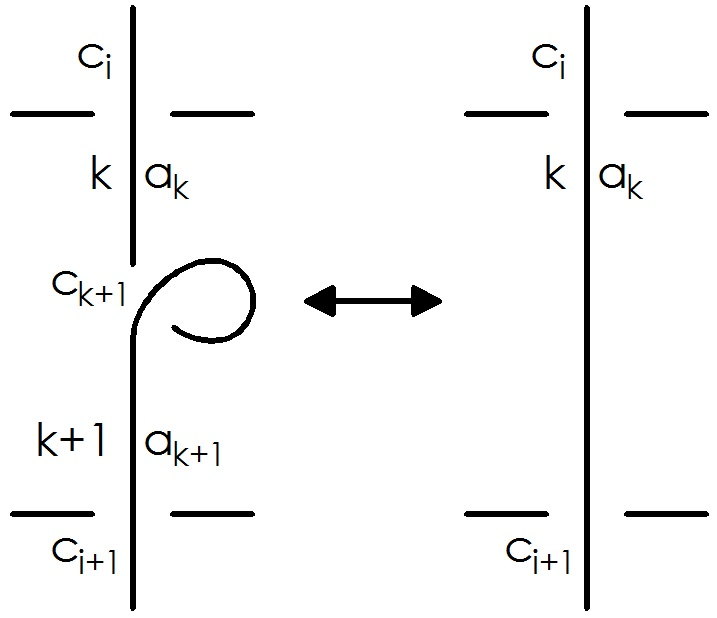
\includegraphics[scale=0.25]{2/Obrazy/R1det}
\end{center}
\end{minipage}
\begin{minipage}{0.5\textwidth}
\begin{center}

			$A'_{+}= \begin{pmatrix}
			${\Huge A}$ & \begin{matrix} a_{1,k} \\ \vdots \\ a_{i,k} \\ 0 \\ \vdots
			\\ 0 \end{matrix} & \begin{matrix} 0 \\ \vdots \\ 0 \\ a_{i+1,k} \\ \vdots
			\\ a_{k-1,k} \end{matrix} \\
			\begin{matrix} a_{k,1} & \cdots & a_{k,k-1} \end{matrix} & 0 & a_{k,k} \\
			\begin{matrix} 0 & \cdots & 0 \end{matrix} & -1 & 1 \\
			\end{pmatrix}$

			
\end{center}
\end{minipage}



\begin{comment}

			$A'_{+}= \begin{pmatrix}
			${\Huge A}$ & \begin{matrix} 0 \\ \vdots \\ 0 \\ 0 \\ \vdots
			\\ 0 \end{matrix} & \begin{matrix} 0 \\ \vdots \\ 0 \\ 0 \\ \vdots
			\\ 0 \end{matrix} \\
			\begin{matrix} 0 & \cdots & 0 \end{matrix} & 0 & 0 \\
			\begin{matrix} 0 & \cdots & 0 \end{matrix} & -1 & 1 \\
			\end{pmatrix}$
\end{comment}

Równania skrzyżowań o indeksach od 1 do i nie zmieniają się. W równaniach skrzyżowań o indeksach większych od i, k-ty kolor zostaje zastąpiony k+1-szym. Ostatni wiersz macierzy wynika z równania $c_{k+1}$ skrzyżowania. Na mocy lematu znaki równań mogą być tak dobrane aby sumowały się one do 0. Co więcej taki dobór znaków jest również właściwy dla macierzy $A_{+}$. Niech $A'$ będzie minorem $A'_{+}$ powstałym poprzez usunięcie ostatniej kolumny i ostatniego wiersza. 

\begin{center}

			$
			A'= \begin{pmatrix}
			${\Huge A}$ & \begin{matrix} a_{1,k} \\ \vdots \\ a_{i,k} \\ 0 \\ \vdots
			\\ 0 \end{matrix} \\
			\begin{matrix} a_{k,1} & \cdots & a_{k,k-1} \end{matrix} & 0 \\
			\end{pmatrix}$
			
\end{center}

Dodając do k-tego wiersza sumę pozostałych wierszy otrzymamy macierz:
\begin{center}

			$\begin{pmatrix}
			${\Huge A}$ & \begin{matrix} a_{1,k} \\ \vdots \\ a_{i,k} \\ 0 \\ \vdots
			\\ 0 \end{matrix} \\
			\begin{matrix} 0 & \cdots & 0 \end{matrix} & 1 \\
			\end{pmatrix}$
			
\end{center}


Stąd korzystając z rozwinięcia Laplace'a względem ostatniego wiersza, $\vert det \big(A'\big) \vert = \vert 1 \times det \big(A\big) \vert$. Przenosząc element $a_{k,k} =1$ w lewy górny róg macierzy i powtarzając rozumowanie z twierdzenia o postaci macierzy diagonalnej, otrzymujemy, że jeśli macierz diagonalna odpowiadająca $A$ ma wartości na głównej przekątnej $\lbrace \vert d_{1} \vert, \cdots, \vert d_{k-1} \vert \rbrace$, to macierz diagonalna odpowiadająca $A'$, ma wartości $\lbrace 1, \vert d_{1} \vert, \cdots, \vert d_{k-1} \vert \rbrace$

\item Drugi ruch Reidemeistera. Bez straty ogólności można założyć że ruch Reidemeistera dotyczy i-tego, oraz k-tego łuku, gdzie i-ty łuk jest łukiem górnym, oraz ruch jest pomiędzy  skrzyżowaniami $ c_{j}, c_{j+1}$. 

\begin{center}
			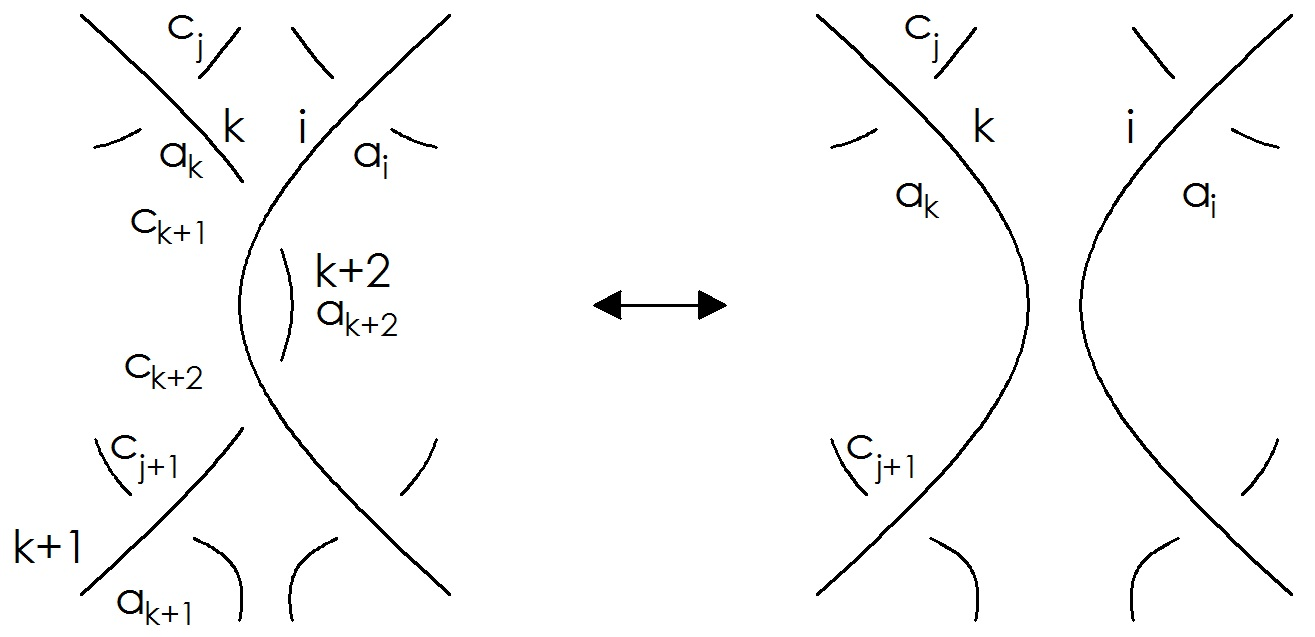
\includegraphics[scale=0.25]{2/Obrazy/R2det}
\end{center}

Niech indeksy skrzyżowań do których dochodzi łuk k są mniejsze od i+1, oraz indeksy skrzyżowań do których dochodzi k+1, są większe od i. Równania skrzyżowań do których nie dochodzi łuk $k+1$ nie zmieniają się. Macierze kolorowania mają zatem postacie:

\begin{center}

			$A'_{+}= \begin{pmatrix}
			${\Huge A}$ & \begin{matrix} a_{1,k} \\ \vdots \\ a_{i,k} \\ 0 \\ \vdots
			\\ 0 \end{matrix} & \begin{matrix} 0 \\ \vdots \\ 0 \\ a_{i+1,k} \\ \vdots
			\\ a_{k-1,k} \end{matrix} & \begin{matrix} 0 \\ \vdots \\ 0 \\ 0 \\ \vdots
			\\ 0 \end{matrix} \\
	 		\\ \begin{matrix} a_{k,1} & \cdots  & a_{k,i}  & \cdots & a_{k,k-1} \end{matrix} & 0 & a_{k,k} & 0
	 		\\ \begin{matrix} 0 & \cdots & 0 & -2 & 0 & \cdots & 0 \end{matrix} & 1 & 0 & 1
			\\ \begin{matrix} 0 & \cdots & 0 & 2 & 0 & \cdots & 0 \end{matrix} & 0 & -1 & -1

			\end{pmatrix}$

	
\end{center}

\begin{center}

			$A'= \begin{pmatrix}
			${\Huge A}$ & \begin{matrix} a_{1,k} \\ \vdots \\ a_{i,k} \\ 0 \\ \vdots
			\\ 0 \end{matrix} & \begin{matrix} 0 \\ \vdots \\ 0 \\ a_{i+1,k} \\ \vdots
			\\ a_{k-1,k} \end{matrix}
	 		\\ \begin{matrix} a_{k,1} & \cdots  & a_{k,i}  & \cdots & a_{k,k-1} \end{matrix} & 0 & a_{k,k}
	 		\\ \begin{matrix} 0 & \cdots & 0 & -2 & 0 & \cdots & 0 \end{matrix} & 1 & 0 


			\end{pmatrix}$

		
\end{center}

Po wykonaniu na macierzy $A'$ następujących operacji: dodanie do ostatniej (k+1) kolumny sumy pozostałych kolumn, oraz dodanie do przedostatniego wiersza (k) sumy wierszy od 1 do k-1, oraz zastosowaniu rozwinięcia Laplace'a otrzymamy $\vert det \big( A' \big) \vert = \vert det \big( A \big) \vert$. Macierz diagonalna ma postać $\lbrace 1, 1, \vert d_{1} \vert, \cdots, \vert d_{k} \vert \rbrace$. Argumentacja jest analogiczna jak w pierwszym ruchu Reidemeistera.
 
 \item Trzeci ruch Reidemeistera. Trzeci ruch nie zmienia liczby skrzyżowań. Macierze $A_{+}$, oraz $A'_{+}$ mają wymiar $k \times k$. Diagram przed i po wykonaniu ruchu, oraz odpowiadające im macierze kolorowań zostały przedstawione poniżej.
 
 \begin{center}
 			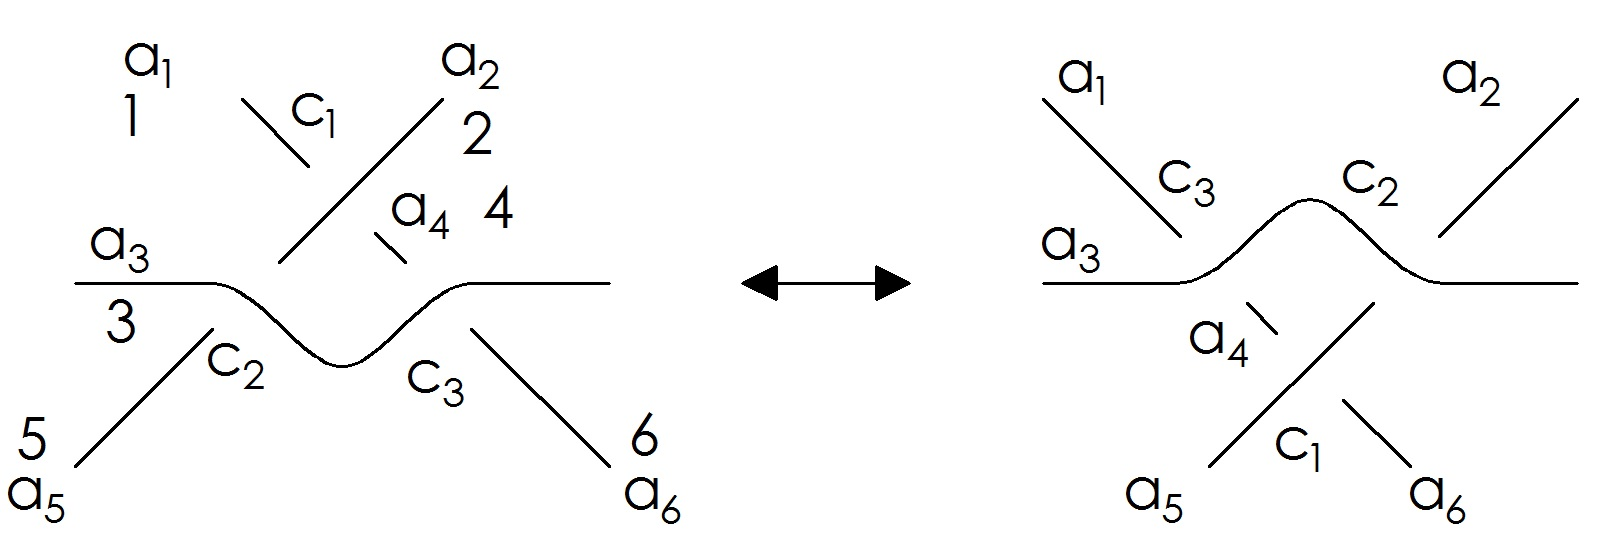
\includegraphics[scale=0.3]{2/Obrazy/R3det}
 \end{center}

\begin{minipage}{0.5\textwidth}
\begin{center}

			$\begin{pmatrix}
			\begin{matrix}
			-1 & 2 & 0 & -1 & 0 & 0 \\
			0 & -1 & -2 & 0 & -1 & 0 \\
			0 & 0 & 2 & -1 & 0 & -1 \\
			\end{matrix} & ${\Huge{0}}$ \\
			${\Huge{$A_{x}$}}$ & ${\Huge{$A_{y}$}}$


			\end{pmatrix}$
			

\end{center}
\end{minipage}
\begin{minipage}{0.5\textwidth}
\begin{center}
			$\begin{pmatrix}
			\begin{matrix}
			0 & 0 & 0 & -1 & 2 & -1 \\
			0 & -1 & -2 & 0 & -1 & 0 \\
			-1 & 0 & 2 & -1 & 0 & 0 \\
			\end{matrix} & ${\Huge{0}}$ \\
			${\Huge{$A_{x}$}}$ & ${\Huge{$A_{y}$}}$


			\end{pmatrix}$
\end{center}
\end{minipage} 

Ponadto łuk $a_4$ występuje jedynie w równaniach skrzyżowań $c_{3}$, oraz $c_{1}$. Wynika stąd ze czwarta kolumna macierzy $A_{x}$ jest równa 0. Niech macierze $A$, oraz $A'$ będą macierzami powstałymi po usunięciu pierwszego wiersza i trzeciej kolumny. Rozważmy ciąg operacji.

\begin{minipage}{0.5\textwidth}

Dla macierzy $A'$:

\begin{itemize}
\item Odjęcie czwartej kolumny od szóstej kolumny,
\item Zamiana pierwszego i drugiego wiersza,
\item Zamiana pierwszej i czwartej kolumny.
\end{itemize}
	

\end{minipage}
\begin{minipage}{0.5\textwidth}

Dla macierzy $A$:
\begin{itemize}
\item Odjęcie czwartej kolumny od pierwszej kolumny,
\item Zamiana pierwszego i drugiego wiersza,
\item Zamiana pierwszej i czwartej kolumny.
\end{itemize}
\end{minipage} 

Wtedy obie macierze zostaną przekształcone do postaci:

\begin{center}
			$\begin{pmatrix}
			\begin{matrix}
			-1 & 0 & 0 & 0 & 0 \\
			0 & -1 & 0 & -1 & 0 \\
			\end{matrix} & ${\Huge{0}}$ \\
			${\Huge{$A'_{x}$}}$ & ${\Huge{$A_{y}$}}$
			\end{pmatrix}$
			
\end{center}

Gdzie, $A'_{x}$ jest macierzą powstałą przez usunięcie trzeciej kolumny z macierzy $A_{x}$. Zatem sprowadzając macierze do postaci diagonalnej otrzymujemy że $det \vert A' \vert = det \vert A \vert $, oraz odpowiadające macierze diagonalne są równe $D'=D$.
\end{enumerate}
\end{proof}



\begin{twierdzenie}
Diagram L może być kolorowalny mod n $\Leftrightarrow \vert det(L) \vert$ oraz n nie są względnie pierwsze.

\end{twierdzenie}

\begin{proof}
Istnienie kolorowania mod n oznacza istnienie kolorów $\lbrace a_{1}, \cdots, a_{k} \rbrace$, takich że równania kolorowań są spełnione dla każdego skrzyżowania. Równoważnie, jest spełnione równanie macierzowe: $ A_{+}x \equiv 0$ mod n, $x \in \Z^k_{n}$. Z lematu wynika, że można przyjąć $a_{1} = 0 $. Ponieważ równania kolorowań są liniowo zależne i $a_{1} = 0 $, zatem powyższa równość zachodzi $\Leftrightarrow Ax' \equiv 0$ mod n, $x' \in \Z^{k-1}_{n}$. \\
Korzystając z twierdzenia o postaci diagonalnej otrzymujemy $A = X^{-1} D Y^{-1}$. \\ $X^{-1}$, $Y^{-1}$ są macierzami całkowitoliczbowymi. Niech $\overline{X^{-1}} = X^{-1}$ mod n, $\overline{Y^{-1}} = Y^{-1}$ mod n, oznacza przypisanie każdemu elementowi macierzy, reszty z dzielenia mod n. Stąd $Ax' \equiv 0 \Leftrightarrow \overline{A}x' \equiv 0 \Leftrightarrow \overline{X^{-1} D Y^{-1}}x' \equiv 0 \Leftrightarrow \overline{X^{-1}} \times \overline{D} \times \overline{Y^{-1}}x' \equiv 0 \Leftrightarrow \overline{D} y' \equiv 0$, $y' =Y^{-1}x'$, $y' \in \Z^{k-1}_{n}$. Ponieważ kolorowanie $x'$ nie jest trywialne, to $y' \neq 0$ mod n. Zatem $\exists i \in \lbrace 1, \cdots, k \rbrace$  $d_{i} \times y'_{i} \neq 0$ mod n. Ponieważ $\forall i \in \lbrace 1, \cdots, k \rbrace$  $y'_{i} \in \Z_{n}$, to $d_{i}$, oraz $n$, nie są względnie pierwsze. Ponadto $\vert det \big(L \big) \vert =\vert det \big(D \big) \vert= \prod^k_{i=1} \vert d_{i}\vert$. Stąd $det \big(L \big)$, oraz $n$ nie są względnie pierwsze.
\end{proof}
\textbf{Wniosek:} 
\begin{itemize}
\item Jeżeli $\vert det \big(L \big) \vert = 0$, to dla każdego n, diagram jest kolorowalny modulo n,
\item Jeżeli $\vert det \big(L \big) \vert = 1$, to dla żadnego n, diagram nie jest. kolorowalny modulo n
\end{itemize}


\subsection{Wyznacznik sumy spójnej} 
Niech $K$, $\tilde{K}$ będą węzłami, $L$, $\tilde{L}$ ich diagramami, $A_{+}$, $\tilde{A_{+}}$ macierzami kolorowania, $C$, $\tilde{C}$ zbiorami skrzyżowań. Rozważmy sumę spójną węzłów $K\#\tilde{K}$. Bez straty ogólności można przyjąć dwa upraszczające założenia:
\begin{itemize}
\item Diagramy zostały połączone względem k-tego łuku w diagramie $L$, oraz względem pierwszego łuku w diagramie $\tilde{L}$.  
\item Skrzyżowania w diagramie $L$ zostały tak ponumerowane że skrzyżowania do których dochodzi łuk k, oraz znajdują się przed miejscem połączenia diagramów mają numer mniejszy od i+1, zaś skrzyżowania znajdujące się za miejscem połączenia mają numer większy od i. Analogicznie dla diagramu $\tilde{L}$. 
\end{itemize} 

\begin{twierdzenie}
Wyznacznik sumy spójnej diagramów $\vert det \big( K\#\tilde{K} \big) \vert = \vert det \big( K \big) \vert \times \vert det \big( \tilde{K} \big) \vert$. Ponadto jeżeli wartości w odpowiadających macierzach diagonalnych wynoszą $\lbrace \vert d_{1} \vert, \cdots, \vert d_{k} \vert \rbrace$, oraz $\lbrace \vert \tilde {  d_{1}} \vert , \cdots,  \vert\tilde{ d_{k}} \vert \rbrace$, to wartości w macierzy diagonalnej dla diagramu sumy spójnej wynoszą $\lbrace 1, \vert d_{1} \vert, \cdots, \vert d_{k} \vert, \vert \tilde {d_{1}} \vert, \cdots, \vert \tilde{d_{k}} \vert\rbrace$.
\end{twierdzenie}

\begin{proof}
Operacja sumy spójnej przerywa dwa wybrane łuki i łączy końce. 
\begin{center}
			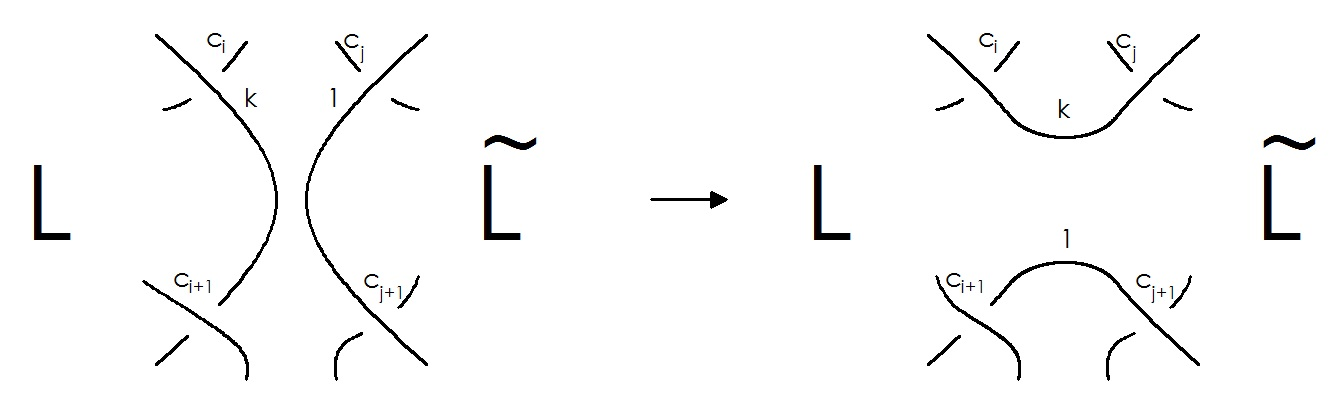
\includegraphics[scale=0.3]{2/Obrazy/Sumaspojna}
\end{center}

W diagramie $L$, równania skrzyżowań o indeksach większych od i zostaną zmienione. Współczynnik odpowiadający łukowi k, będzie odpowiadał łukowi pierwszemu z diagramu $\tilde{L}$. W diagramie $\tilde{L}$, współczynnik odpowiadający łukowi pierwszemu będzie odpowiadał łukowi k z diagramu $L$. Macierz kolorowania ma postać: \\
\begin{center}

$\big( A_{L\#\tilde{L}}\big)_{+}= \begin{pmatrix} 

\begin{matrix}
a_{1,1} & \cdots & a_{1,k-1} \\
\vdots & \ddots & \vdots \\
a_{i,1} & \cdots & a_{i,k-1} \\
a_{i+1,1} & \cdots & a_{i+1,k-1} \\
\vdots & \ddots & \vdots \\
a_{k,1} & \cdots & a_{k,k-1} \\
\end{matrix}

&
\begin{matrix}
a_{1,k}\\
\vdots\\
a_{i,k}\\
0\\
\vdots\\
0
\end{matrix}
&
\begin{matrix}
0\\
\vdots\\
0\\
a_{i+1,k}\\
\vdots\\
a_{k,k}

\end{matrix}
&
${\Huge{0}}$


\\
${\Huge{0}}$
&
\begin{matrix}
\tilde{a}_{1,1}\\
\vdots\\
\tilde{a}_{\tilde{i},1}\\
0\\
\vdots\\
0
\end{matrix}
&
\begin{matrix}
0\\
\vdots\\
0\\
\tilde{a}_{\tilde{i}+1,1}\\
\vdots\\
\tilde{a}_{k,1}

\end{matrix}
&
\begin{matrix}
\tilde{a}_{1,2} & \cdots & \tilde{a}_{1,k} \\
\vdots & \ddots & \vdots \\
\tilde{a}_{\tilde{i},2} & \cdots & \tilde{a}_{\tilde{i},k} \\
\tilde{a}_{\tilde{i}+1,2} & \cdots & \tilde{a}_{\tilde{i}+1,k} \\
\vdots & \ddots & \vdots \\
\tilde{a}_{k,2} & \cdots & \tilde{a}_{k,k} \\
\end{matrix}

\end{pmatrix}$
\end{center}
Po usunięciu z macierzy k+1-szego wiersza oraz k+1-szej kolumny otrzymamy 
\begin{center}

$ A_{L\#\tilde{L}}= \begin{pmatrix} 

\begin{matrix}
a_{1,1} & \cdots & a_{1,k-1} \\
\vdots & \ddots & \vdots \\
a_{i,1} & \cdots & a_{i,k-1} \\
a_{i+1,1} & \cdots & a_{i+1,k-1} \\
\vdots & \ddots & \vdots \\
a_{k,1} & \cdots & a_{k,k-1} \\
\end{matrix}

&
\begin{matrix}
a_{1,k}\\
\vdots\\
a_{i,k}\\
0\\
\vdots\\
0
\end{matrix}

&
${\Huge{0}}$


\\
${\Huge{0}}$
&
\begin{matrix}
\tilde{a}_{2,1}\\
\vdots\\
\tilde{a}_{\tilde{i},1}\\
0\\
\vdots\\
0
\end{matrix}

&
\begin{matrix}
\tilde{a}_{2,2} & \cdots & \tilde{a}_{2,k} \\
\vdots & \ddots & \vdots \\
\tilde{a}_{\tilde{i},2} & \cdots & \tilde{a}_{\tilde{i},k} \\
\tilde{a}_{\tilde{i}+1,2} & \cdots & \tilde{a}_{\tilde{i}+1,k} \\
\vdots & \ddots & \vdots \\
\tilde{a}_{k,2} & \cdots & \tilde{a}_{k,k} \\
\end{matrix}

\end{pmatrix}$
\end{center}
Następnie dodając do $k$-tego wiersza sumę wierszy od $1$ do $k-1$, oraz zamieniając $k$-ty wiersz z $k+\tilde{k}$-szym wierszem i $k$-tą kolumnę z $k+\tilde{k}$ kolumną mamy:


\begin{center}

$ A_{L\#\tilde{L}}= \begin{pmatrix} ${\Huge{A}}$ & ${\Huge{0}}$ &
\begin{matrix}
0\\
\vdots\\
0
\end{matrix} \\

${\Huge{0}}$ & ${\Huge{$\tilde{A}$}}$ & \begin{matrix}
0\\
\vdots\\
0
\end{matrix}  \\

\begin{matrix}
0 & \cdots & 0
\end{matrix} 
&
\begin{matrix}
0 & \cdots & 0
\end{matrix} 
&
\sum_{m=1}^i a_{m,k}

\end{pmatrix}
   $ 
    
\end{center}

Na podstawie wniosku o szachownicy diagramu $\sum_{m=1}^i a_{m,k}=\mp 1$. Zatem $\vert det \big(A_{L\#\tilde{L}} \big) \vert = 1 \times \vert det \big(A_{L} \big) \vert \times \vert det \big(A_{\tilde{L}} \big) \vert$. 
Ponadto przesuwając 1 w lewy górny róg macierzy i stosując proces diagonalizacji otrzymamy, że elementami macierzy diagonalnej są $\lbrace 1, \vert d_{1} \vert, \cdots, \vert d_{k} \vert,  \vert \tilde {d_{1}} \vert, \cdots, \vert \tilde{d_{k}}  \vert \rbrace$.

\end{proof}



\subsection{Grupy kolorowań}
\begin{definicja}
Grupa kolorowań diagramu Col(L), to grupa abelowa, w której generatorami są łuki diagramu, zaś relacjami są równania kolorowań, oraz ustalony koloru wybranego łuku, $a_{1} = 0$.\\ Formalnie: $Col(L)=\langle a_{1}, \cdots, a_{k} \big\vert \begin{pmatrix}
a_{j_{1}} + a_{j_{2}} - 2\times a_{j_{3}} \equiv 0 \\
\vdots \\
a_{j_{k-2}} + a_{j_{k-1}} - 2\times a_{j_{k}} \equiv 0
\end{pmatrix}, a_{1} = 0 \rangle$. \\
$Col(L) = \langle x \big\vert Ax \equiv 0 \rangle$, $x \in \Z^{k-1}$ \\
\end{definicja}

Grupa kolorowań nie jest dobrze zdefiniowanym pojęciem. Zależy ona bowiem od sposobu indeksowania łuków, skrzyżowań oraz wyboru koloru dla pierwszego elementu. 

\begin{twierdzenie}
Skończenie generowana grupa przemienna jest izomorficzna z produktem grup cyklicznych.
\end{twierdzenie}
Grupa kolorowań ma zatem postać: $Col(L) \cong \prod_{i=1}^m \Z_{n_{i}}$. \\
Z definicji grupy wynika że $Col(L) \cong \Z^m/\big(A\Z^m\big)$. Niech $A=X^{-1}DY^{-1}$ \\
$\Z^m/\big(A\Z^m\big) \cong \Z^m/\big(X^{-1}DY^{-1}\Z^m\big)  \cong \Z^m/\big(D\Z^m\big) \cong \Z^m/\big(\prod_{i=1}^m \vert d_{i} \vert \Z\big) \cong \prod_{i=1}^m \Z_{\vert d_{i} \vert}$ 

Klasa izomorfizmów grupy jest dobrze zdefiniowana. Wyznacznik, oraz wartości w macierzy diagonalnej nie zależą od wyboru diagramu, sposobu indeksowania łuków ani skrzyżowań. Produkt grup cyklicznych izomorficzny z grupą kolorowania jest niezmiennikiem węzła. \\
\textbf{Wniosek:} Grupa kolorowań jest nieskończona $\Leftrightarrow$ $det(\big(L\big) = 0$.


\subsection{Przykład zastosowań - rodzina węzłów}
\textbf{Przykład 1:}
Rozważmy następującą rodzinę węzłów $K_{k}$, $k \geq 3 $. Korzystając z własności kolorowań wykażemy że dla różnych k, diagramy przedstawiają różne węzły. 
\begin{center}
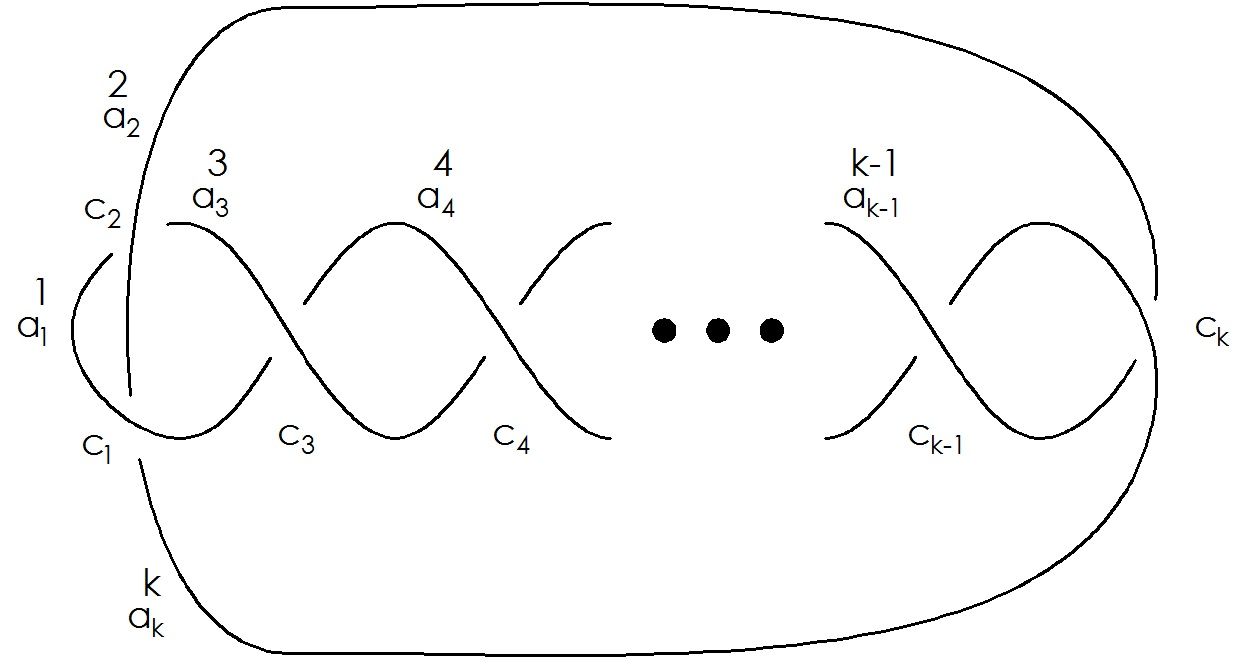
\includegraphics[scale=0.3]{2/Obrazy/Wezelprzyklad} \\
\end{center}
Macierz kolorowania ma postać:
\begin{center}


$A_{k+}=\bordermatrix{
~       &  1 &  2 &  3 &  4 &  5 & \cdots & k-2  &  k-1 &  k \cr
c_{1}   &  2 & -1 &  0 &  0 &  0 & \cdots &  0   &  0   & -1 \cr
c_{2}   & -1 &  2 & -1 &  0 &  0 & \cdots &  0   &  0   &  0 \cr
c_{3}   & -1 &  0 &  2 & -1 &  0 & \cdots &  0   &  0   &  0 \cr
c_{4}   &  0 &  0 & -1 &  2 & -1 & \cdots &  0   &  0   &  0 \cr
c_{5}   &  0 &  0 &  0 & -1 &  2 & \cdots &  0   &  0   &  0 \cr
\vdots  &  \vdots &  \vdots &  \vdots &  \vdots &  \vdots & \ddots &  \vdots   & \vdots   &  \vdots \cr
c_{k-2} &  0 &  0 &  0 &  0 &  0 & \cdots &  2   & -1   &  0 \cr
c_{k-1} &  0 &  0 &  0 &  0 &  0 & \cdots &  -1  &  2   & -1 \cr
c_{k}   &  0 & -1 &  0 &  0 &  0 & \cdots &  0   & -1   &  2 \cr}
$


\end{center}

Rozważmy macierz A, powstałą po usunięciu ostatniej kolumny i ostatniego wiersza. Za pomocą operacji wierszowych i kolumnowych, macierz zostanie sprowadzona do postaci diagonalnej.
\begin{center}

$A_{k}=\begin{pmatrix}
2  & -1 &  0 & 0 & 0 & 0 & \cdots & 0 & 0 & 0 \\
-1 &  2 & -1 & 0 & 0 & 0 & \cdots & 0 & 0 & 0 \\
-1 &  0 &  2 &-1 & 0 & 0 & \cdots & 0 & 0 & 0 \\
 0 &  0 & -1 & 2 &-1 & 0 & \cdots & 0 & 0 & 0 \\
 0 &  0 &  0 &-1 & 2 &-1 & \cdots & 0 & 0 & 0 \\
 \vdots  &  \vdots &  \vdots &  \vdots &  \vdots &  \vdots & \ddots &  \vdots   & \vdots   &  \vdots\\
 0 &  0 &  0 & 0 & 0 & 0 & \cdots &-1 & 2 &-1 \\
 0 &  0 &  0 & 0 & 0 &0  & \cdots & 0 &-1 & 2 \\
\end{pmatrix}$

\end{center}
Dodając do pierwszej kolumny, podwojoną drugą kolumnę, zamieniając pierwszą i drugą kolumnę miejscami, oraz dodając do drugiego wiersza podwojony pierwszy wiersz otrzymujemy. 
 \begin{center}
 

$A_{k}^{1} = \begin{pmatrix}
-1 &  0 &  0 & 0 & 0 & 0 & \cdots & 0 & 0 & 0 \\
 0 &  3 & -1 & 0 & 0 & 0 & \cdots & 0 & 0 & 0 \\
 0 & -1 &  2 &-1 & 0 & 0 & \cdots & 0 & 0 & 0 \\
 0 &  0 & -1 & 2 &-1 & 0 & \cdots & 0 & 0 & 0 \\
 0 &  0 &  0 &-1 & 2 &-1 & \cdots & 0 & 0 & 0 \\
 \vdots  &  \vdots &  \vdots &  \vdots &  \vdots &  \vdots & \ddots &  \vdots   & \vdots   &  \vdots\\
 0 &  0 &  0 & 0 & 0 & 0 & \cdots &-1 & 2 &-1 \\
 0 &  0 &  0 & 0 & 0 &0  & \cdots & 0 &-1 & 2 \\
\end{pmatrix}$
 \end{center}
 

 Niech W będzie macierzą $n \times n$, taką że na głównej przekątnej znajdują się 2, oraz bezpośrednio nad i pod główną przekątną znajdują się -1. \\
 \begin{center}
 

 $
 W_{n}=\begin{pmatrix}
2 & -1 & 0 & \cdots & 0 \\
-1& 2 & -1 & \cdots & 0 \\
0 &-1 &  2 & \cdots & 0 \\
\vdots & \vdots & \vdots & \ddots & \vdots \\
0 & 0 & 0 &\cdots & 2 \\
 \end{pmatrix}
 $ \\
  \end{center}
 Wtedy istnieje ciąg operacji:
\begin{itemize}
\item Zamiana pierwszej i drugiej kolumny
\item Dodanie do drugiej kolumny $2m+1$ krotności pierwszej kolumny.
\item Odjęcie pierwszego wiersza od trzeciego wiersza
\end{itemize}
Przekształca macierz $H_{1}$ w macierz $H_{2}$:

 
	\begin{minipage}{0.5\textwidth}
	\begin{center}
	
	  $H_{1} = \begin{pmatrix}
 2m+1 & \begin{matrix}
 -1 & 0 &\cdots & 0
 \end{matrix} \\
 \begin{matrix}
 -2m+1
 \\ 0 \\ \vdots \\ 0
 \end{matrix} & ${\Large{$W_{n}$}}$
 
 
 \end{pmatrix}$ \\
\end{center} 
 \end{minipage}
 \begin{minipage}{0.5\textwidth}
 \begin{center}
 $H_{2} = \begin{pmatrix}
 -1 & 0 & \begin{matrix}
 0 & 0 &\cdots & 0
 \end{matrix} \\
 0 & 2m+3 & \begin{matrix}
 -1 & 0 &\cdots & 0
 \end{matrix} \\
 \begin{matrix}
 0 
 \\ 0 \\ \vdots \\ 0
 \end{matrix} &
 \begin{matrix}
 -2m-1
 \\ 0 \\ \vdots \\ 0
 \end{matrix} & ${\Large{$W_{n-1}$}}$
 
 \end{pmatrix}$ \\
 \end{center} 
 \end{minipage}
Macierz $A_{k}^{1}$ ma postać: \\
\begin{center}

	  $A_{k}^{1} = \begin{pmatrix}
 -1 & 0 &  \begin{matrix}
 0 & 0 &\cdots & 0
 \end{matrix} \\ 
 0 & 3 & \begin{matrix}
 -1 & 0 &\cdots & 0
 \end{matrix}
 \\
 
 \begin{matrix}
 0
 \\ 0 \\ \vdots \\ 0
 \end{matrix} & \begin{matrix}
 -1 \\ 0 \\ \vdots \\ 0
 \end{matrix} & ${\Large{$W_{k-3}$}}$
 
 
 \end{pmatrix}$ \\

\end{center}
Powtarzając ciąg operacji powyżej mamy:

\begin{center}
	  $A_{k}^{i} = \begin{pmatrix}
 -1 & 0 & \cdots & 0 & 0 &  \begin{matrix}
 0 & 0 &\cdots & 0
 \end{matrix} \\ 
 0 & -1 & \cdots  & 0 & 0 &  \begin{matrix}
 0 & 0 &\cdots & 0
 \end{matrix} 
 \\
 \vdots & \vdots & \ddots & \vdots & \vdots & \begin{matrix}
 \vdots & \vdots &\ddots & \vdots
 \end{matrix} 
 \\ 
  0 & 0 & \cdots  & -1 & 0 &  \begin{matrix}
 0 & 0 &\cdots & 0 \end{matrix}
 \\
 0 & 0 & \cdots & 0 & 2i+1  & \begin{matrix}
 -1 & 0 &\cdots & 0
 \end{matrix}
 \\
 
 \begin{matrix}
 0
 \\ 0 \\ \vdots \\ 0
 \end{matrix} &  \begin{matrix}
 0
 \\ 0 \\ \vdots \\ 0
 \end{matrix}
 & \begin{matrix}
 \cdots
 \\ \cdots \\ \ddots \\ \cdots
 \end{matrix}
 &
 \begin{matrix}
 0
 \\ 0 \\ \vdots \\ 0
 \end{matrix} &
  \begin{matrix}
 -2i+1 \\ 0 \\ \vdots \\ 0
 \end{matrix} & ${\Large{$W_{k-2-i}$}}$
 
 
 \end{pmatrix}$ \\


\end{center}

Stąd macierz $A_{k} $ może zostać przekształcona do postaci diagonalnej takiej że na głównej przekątnej znajdują się elementy $\lbrace -1, -1, \cdots, -1, 2k-3 \rbrace$. Stąd $\vert det \big( L_{k} \big) \vert = 2k - 3$. Ponieważ wyznacznik diagramu jest niezmiennikiem węzła to dla każdego k, diagram przedstawia różne węzły. \\ \\

 \textbf{Przykład 2:}
 Niech $K'_{k}$ będą tymi węzłami z poprzedniego przykładu że, wyznacznik diagramu jest pewną potęgą 3. Czy dla pewnego $k\geq9$, $K_{k}$  jest sumą spójną pewnej, większej od 1, liczby trójlistników? \\ \\
 Z poprzedniego twierdzenia wyznacznik splotu węzłów, jest iloczynem wyznaczników diagramów. Zatem splot n trójlistników ma wyznacznik $3^n$. Wobec tego istnieje węzeł $K'_{k}$, że wyznacznik jego diagramu jest równy wyznacznikowi splotu trójlistników. Z twierdzenia wiadomo również że struktura macierzy diagonalnej jest niezmiennikiem węzła. Macierz diagonalna odpowiadająca $L_{k}$, ma na głównej przekątnej wartości $\lbrace 1, 1, \cdots, 1, 3^n_{k} \rbrace$, zaś macierz diagonalna odpowiadająca diagramowi splotu trójlistników ma wartości $\lbrace 1, \cdots, 1, 3, \cdots, 3 \rbrace$. Ponadto wartości w obu macierzach diagonalnych spełniają warunek $d_{i} \vert d_{i+1}$, więc macierze diagonalna tej postaci są jedyne. Stąd żaden splot trójlistników nie jest węzłem postaci $K_{k}$.
 

 